\chapter{XÁC ĐỊNH VÀ TÍCH HỢP AI ĐÚNG PHẠM VI}

\section{AI nằm ở đâu trong hệ thống}

AI nằm trong module \texttt{services/ai\_service.py}, phía sau backend Python và sau bước lấy dữ liệu từ SQL. Người dùng không gọi trực tiếp nhà cung cấp model. Backend kiểm tra quyền, chọn bản ghi context, dựng prompt, gọi adapter, kiểm tra output rồi mới trả kết quả về giao diện.

\begin{figure}[h!]
\centering
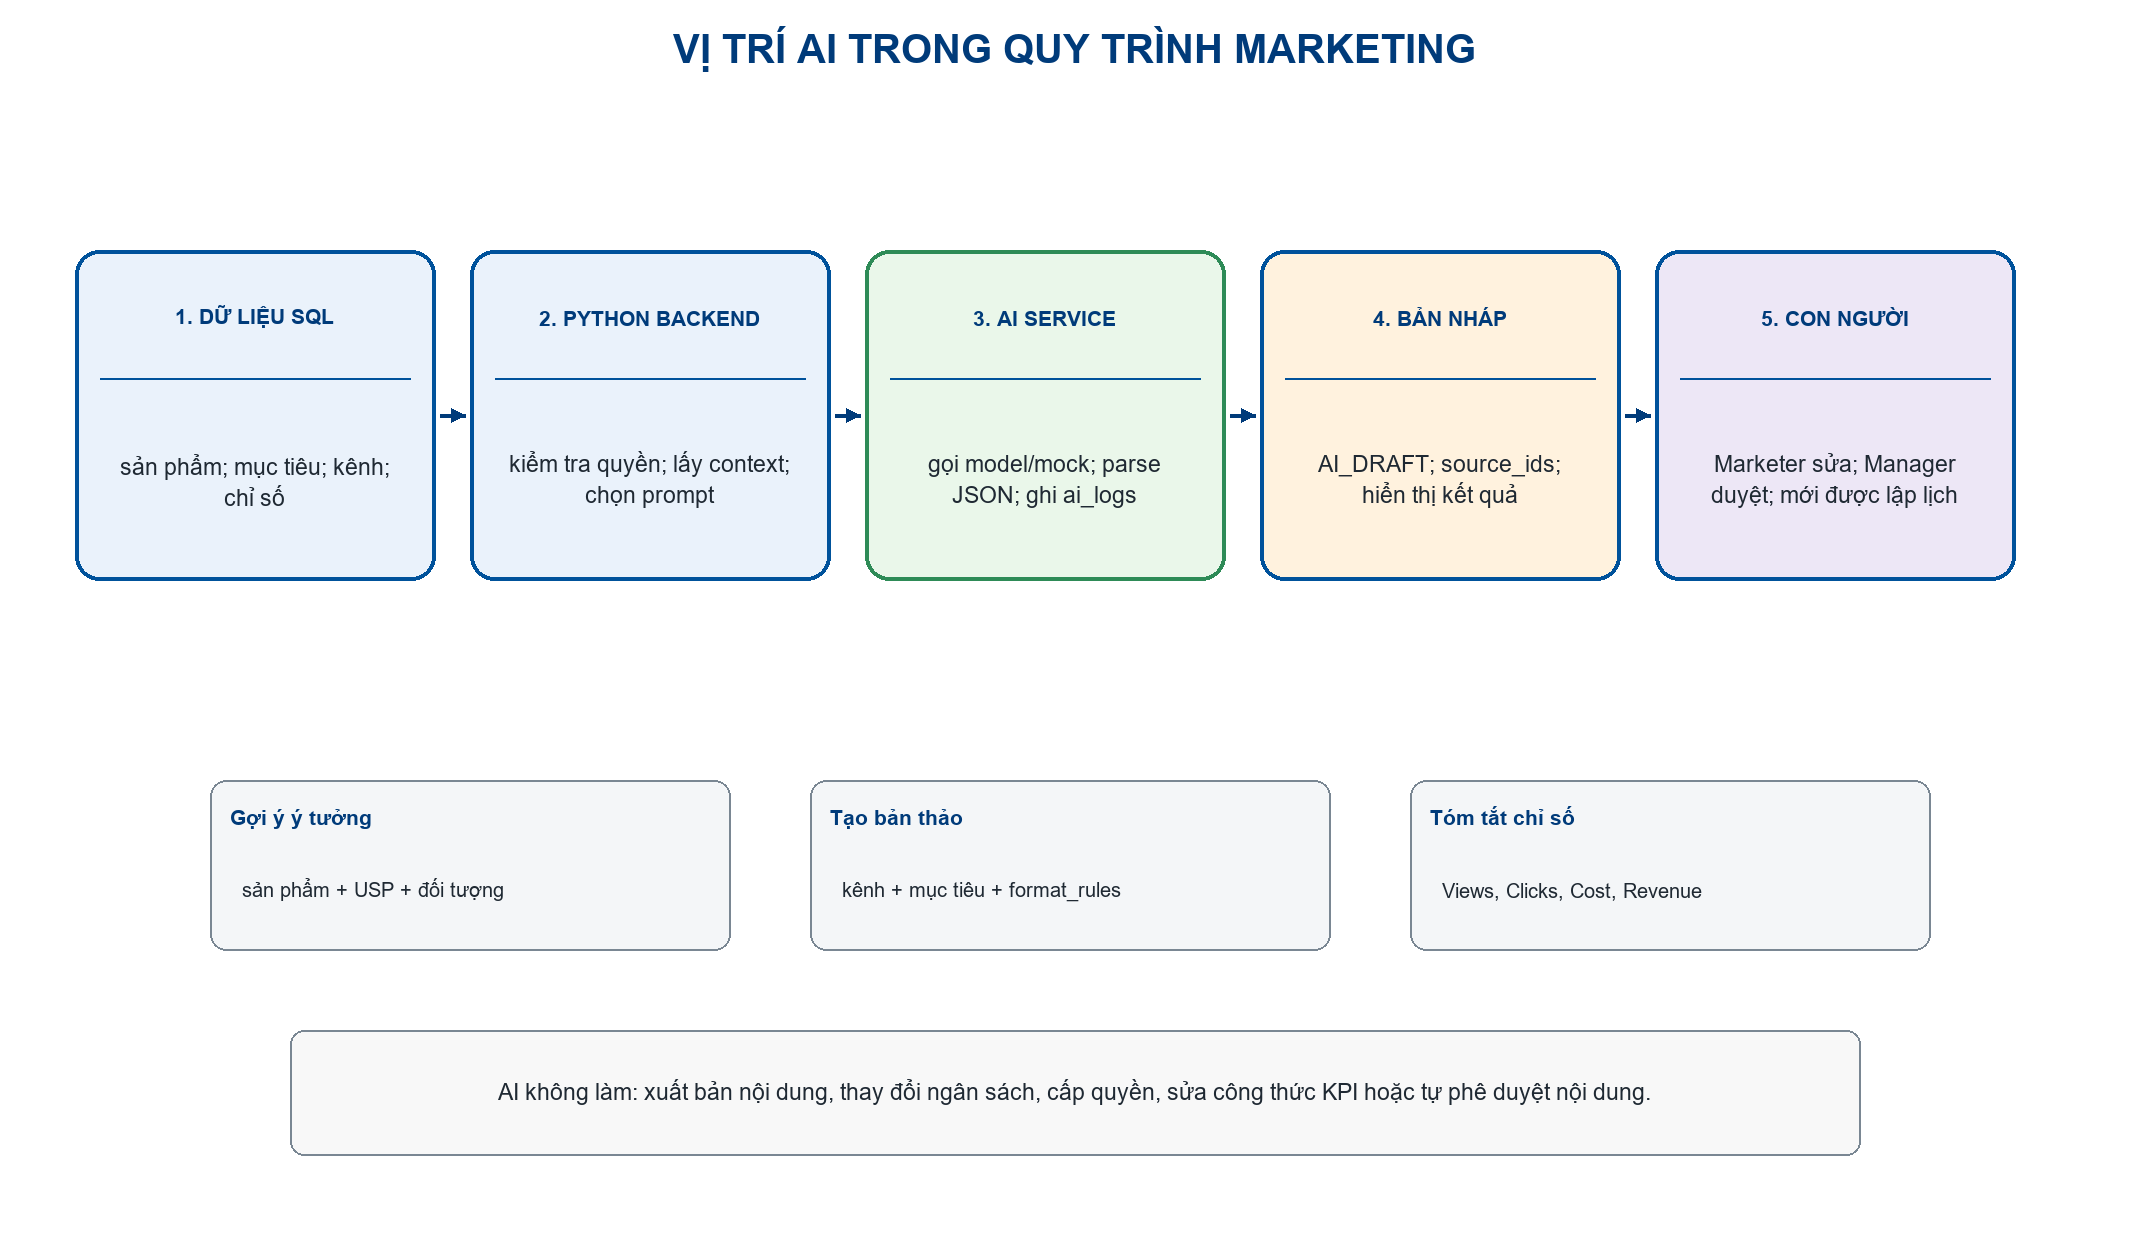
\includegraphics[width=\textwidth]{images/ai_flow.png}
\caption{Vị trí và luồng xử lý của AI trong hệ thống}
\end{figure}

\begin{table}[h!]
\centering
\small
\caption{Những việc AI được làm và không được làm}
\begin{tabularx}{\textwidth}{|L{3.4cm}|Y|Y|}
\hline
\textbf{Phạm vi} & \textbf{AI được làm} & \textbf{AI không được làm}\\\hline
Nội dung & Gợi ý ý tưởng và tạo bản nháp theo sản phẩm, mục tiêu, kênh. & Tự xuất bản hoặc thay đổi bản nháp đã được Manager duyệt.\\\hline
Báo cáo & Tóm tắt số liệu đã lọc và nêu điểm cần xem xét. & Tự tính thay công thức KPI hoặc tạo số liệu không có trong CSDL.\\\hline
Quy trình & Đề xuất câu chữ, lý do hoặc bước cần kiểm tra. & Cấp quyền, đổi ngân sách, đổi trạng thái duyệt hoặc tạo lịch không có xác nhận.\\\hline
\end{tabularx}
\end{table}

\section{Ba nhiệm vụ AI trong chủ đề}

\begin{table}[h!]
\centering
\small
\caption{Ba nhiệm vụ AI, dữ liệu vào và kết quả ra}
\begin{tabularx}{\textwidth}{|L{2.8cm}|L{4.4cm}|Y|Y|}
\hline
\textbf{Mã} & \textbf{Nhiệm vụ} & \textbf{Đầu vào từ SQL} & \textbf{Đầu ra và điều kiện}\\\hline
AI01 & Gợi ý ý tưởng nội dung & Tên sản phẩm, USP, audience, mục tiêu chiến dịch, kênh. & Ba góc tiếp cận; người dùng chọn trước khi tạo bản nháp.\\\hline
AI02 & Tạo bản thảo theo kênh & Sản phẩm, mục tiêu, \texttt{format\_rules}, yêu cầu cụ thể. & JSON gồm headline, body, CTA, hashtags, source\_ids; lưu AI\_DRAFT.\\\hline
AI03 & Tóm tắt báo cáo & Views, Clicks, Conversions, Cost, Revenue đã lọc. & Nhận xét, điểm bất thường và đề xuất; mỗi nhận xét phải có số liệu nguồn.\\\hline
\end{tabularx}
\end{table}

Ba nhiệm vụ trên phục vụ các màn hình Nội dung và Báo cáo. Chúng không thay thế các chức năng quản lý P01--P24. Nếu không có dữ liệu sản phẩm, mục tiêu hoặc số liệu, backend phải báo thiếu dữ liệu thay vì yêu cầu AI tự đoán.

\section{System prompt, User prompt và output schema}

Prompt được tách thành bốn phần để phân biệt luật hệ thống, yêu cầu cụ thể, dữ liệu nguồn và định dạng đầu ra:

\begin{lstlisting}[language={},caption={Prompt mẫu cho AI02}]
SYSTEM:
You are a marketing assistant inside a Python application.
Use only the supplied context. Do not invent claims or metrics.
Return one JSON object. Do not publish or approve content.

USER:
Create a draft for channel={{channel}} and objective={{objective}}.

CONTEXT:
product_name={{name}}; usp={{usp}}; audience={{audience}}
channel_rules={{format_rules}}; source_ids={{source_ids}}

OUTPUT:
{"headline":"string","body":"string","cta":"string",
 "hashtags":["string"],"source_ids":["string"]}
\end{lstlisting}

Backend dùng Pydantic schema để kiểm tra các khóa bắt buộc, kiểu dữ liệu, độ dài theo kênh và \texttt{source\_ids}. Output có markdown fence, thiếu khóa hoặc chứa trường ngoài schema bị từ chối. Bản nháp trước đó được giữ nguyên để người dùng có thể thử lại.

\section{Grounding từ CSDL}

Grounding được thực hiện bằng cách truy vấn đúng chiến dịch, sản phẩm và kênh; sau đó tạo một context whitelist. Không đưa toàn bộ CSDL hoặc thông tin xác thực vào prompt.

\begin{table}[h!]
\centering
\small
\caption{Các trường được phép đưa vào context AI}
\begin{tabularx}{\textwidth}{|L{3.5cm}|Y|Y|}
\hline
\textbf{Nguồn} & \textbf{Trường được phép} & \textbf{Mục đích}\\\hline
\texttt{products} & name, usp, audience, price & Mô tả sản phẩm và khách hàng mục tiêu.\\\hline
\texttt{campaigns} & name, objective, start\_date, end\_date & Xác định mục tiêu và phạm vi chiến dịch.\\\hline
\texttt{marketing\_channels} & name, format\_rules & Giới hạn định dạng và cách trình bày.\\\hline
\texttt{campaign\_metrics} & views, clicks, conversions, cost, revenue, metric\_date & Tóm tắt báo cáo và nhận diện điểm bất thường.\\\hline
\end{tabularx}
\end{table}

\texttt{password\_hash}, JWT secret, API key, token và dữ liệu không liên quan không được đưa vào context. Mỗi kết quả AI lưu \texttt{source\_ids}, \texttt{provider}, \texttt{prompt\_version} và \texttt{result\_status} trong \texttt{ai\_logs}.

\section{Kiểm duyệt của con người}

\begin{enumerate}
  \item Marketer chọn chiến dịch và kênh; backend kiểm tra quyền và lấy context.
  \item AI trả kết quả; backend kiểm tra schema; hệ thống lưu bản nháp AI\_DRAFT.
  \item Marketer đọc nguồn, sửa câu chữ và gửi PENDING.
  \item Manager kiểm tra nội dung, mục tiêu và nguồn context; chỉ Manager mới chuyển APPROVED hoặc REJECTED.
  \item Chỉ nội dung APPROVED mới được lập lịch. AI không có quyền đi tắt bước này.
\end{enumerate}

\section{Quản lý khóa và cấu hình Python}

Cấu hình được đọc từ biến môi trường hoặc secret store. Mã nguồn chỉ khai báo tên biến; không ghi khóa thật vào báo cáo, log hoặc repository. Mô hình cấu hình dùng Pydantic Settings theo tài liệu chính thức \cite{pydantic}. Cơ chế Bearer/JWT của API tham khảo hướng dẫn FastAPI \cite{fastapi}; mật khẩu người dùng phải lưu dưới dạng băm phù hợp theo khuyến nghị OWASP \cite{owasp}.

\begin{lstlisting}[language=Python,caption={Cấu hình AI không chứa khóa thật}]
from pydantic_settings import BaseSettings, SettingsConfigDict

class Settings(BaseSettings):
    model_config = SettingsConfigDict(env_file=".env", extra="ignore")
    jwt_secret: str
    ai_provider: str = "mock"
    ai_api_key: str | None = None
    ai_model: str = "model-name"
    ai_timeout_seconds: int = 15

settings = Settings()
\end{lstlisting}

\texttt{AI\_PROVIDER=mock} dùng cho chạy local và kiểm thử offline. Khi dùng provider thật, request có timeout, giới hạn retry và mã truy vết; log không được ghi API key.

\section{Xử lý lỗi AI}

\begin{table}[h!]
\centering
\small
\caption{Ma trận lỗi và cách bảo toàn dữ liệu}
\begin{tabularx}{\textwidth}{|L{3.0cm}|C{2.0cm}|Y|}
\hline
\textbf{Tình huống} & \textbf{Phản hồi} & \textbf{Xử lý}\\\hline
Thiếu context & 400 & Báo trường còn thiếu; không gọi model.\\\hline
Timeout & 503 & Giữ bản nháp cũ, ghi log và cho phép thử lại.\\\hline
429/rate limit & 503 & Backoff tối đa hai lần; không tạo bản ghi trùng.\\\hline
JSON sai schema & 502 & Từ chối output; lưu lỗi rút gọn, không ghi đè bản nháp.\\\hline
Provider offline & 503 hoặc mock & Hiển thị nhãn mock; không tự tạo lịch.\\\hline
Thiếu API key & 500 cấu hình & Dừng luồng AI và hướng dẫn cấu hình; không in khóa.\\\hline
\end{tabularx}
\end{table}

\section{Đánh giá thử nghiệm prompt}

Phần này quy định cách thử ba vòng trên cùng một tập yêu cầu mẫu. Thời gian tính từ lúc gửi request đến khi parse được JSON; tỷ lệ hợp lệ là số kết quả parse được chia cho tổng số request. Bảng dưới là mẫu ghi nhận, chưa phải kết quả đã xác nhận; khi nộp phải thay bằng log thật nếu nhóm đã chạy.

\begin{table}[h!]
\centering
\small
\caption{So sánh ba vòng thiết kế prompt trên tập mẫu}
\begin{tabularx}{\textwidth}{|C{1.0cm}|L{4.3cm}|C{2.0cm}|C{2.0cm}|Y|}
\hline
\textbf{Vòng} & \textbf{Thay đổi} & \textbf{Chỉ số phải ghi} & \textbf{Tiêu chí chấp nhận} & \textbf{Trạng thái}\\\hline
1 & Prompt tự do, context nguyên khối, chưa có schema chặt & Thời gian, số lỗi trường và lỗi nội dung & Ghi rõ lỗi làm cơ sở sửa prompt & Chưa đo\\\hline
2 & Giới hạn context, thêm schema và ví dụ JSON & Thời gian, tỷ lệ parse và số timeout & Không dùng output thiếu trường & Chưa đo\\\hline
3 & Tách system/user, whitelist, parser và retry giới hạn & source\_ids, tỷ lệ parse, timeout và số lần cần sửa & Chỉ dùng sau khi parse và có người duyệt & Chưa đo\\\hline
\end{tabularx}
\end{table}

\section{Nhật ký sử dụng AI trong quá trình xây dựng dự án}

\begin{table}[h!]
\centering
\small
\caption{AI được dùng để hỗ trợ, nhóm kiểm tra lại bằng quy tắc nào}
\begin{tabularx}{\textwidth}{|L{3.3cm}|Y|Y|}
\hline
\textbf{Công việc} & \textbf{Gợi ý từ AI} & \textbf{Kiểm tra của nhóm}\\\hline
Phân rã nghiệp vụ & Gợi ý nhóm chức năng quản lý marketing. & Đối chiếu lại với danh mục P01--P26 và actor.\\\hline
Thiết kế CSDL & Gợi ý quan hệ sản phẩm--chiến dịch--nội dung. & Viết DDL, thêm PK/FK/CHECK và chạy thử dữ liệu sai.\\\hline
Viết service Python & Gợi ý cấu trúc router/service. & Đối chiếu quyền, trạng thái, lỗi HTTP và ca kiểm thử.\\\hline
Thiết kế prompt & Gợi ý tách context và schema. & Whitelist trường SQL, parse JSON và bắt buộc HITL.\\\hline
Rà soát mã nguồn & Gợi ý phát hiện lỗi ở RBAC, trạng thái và xử lý ngoại lệ. & Chạy lại ca kiểm thử, đối chiếu DDL và kiểm tra thủ công trước khi chấp nhận.\\\hline
\end{tabularx}
\end{table}

\section{Kết luận chương}

AI được xác định rõ là mô-đun hỗ trợ nằm sau Python backend. AI nhận context từ SQL, thực hiện ba nhiệm vụ có giới hạn và trả kết quả để người dùng kiểm tra. Quyền, ngân sách, công thức KPI, trạng thái duyệt và xuất bản vẫn do Python/SQL cùng người dùng có thẩm quyền kiểm soát.
